\documentclass[a4paper,11pt]{article}
\usepackage[utf8]{inputenc}
\usepackage{amsmath, amssymb, booktabs, enumitem, graphicx}

\title{TME - Semaines 1 à 3}
\author{Yuxiang Zhang \and Antoine Lecomte}
\date{}

\begin{document}

\maketitle

\section*{Partie 1 : Problème et affectation}

\subsection*{Question 2}

Nous avons différentes possibilités pour optimiser les performances de l'algorithme de Gale-Shapley en ce qui concerne les structures de données :

Nous utilisons plusieurs structures de données qui ont chacune des avantages pour les optimisations que nous cherchons à effectuer.

\section{Algorithme \texttt{gale\_shapley\_etudiants}}

\subsection{Structures de données utilisées}
\begin{itemize}
    \item \textbf{\texttt{deque} (double-ended queue) pour \texttt{etudiants\_libres}}
    \begin{itemize}
        \item Permet une gestion efficace des étudiants libres avec un accès en $O(1)$ pour les ajouts/suppressions en tête.
        \item Utilisé pour traiter rapidement les étudiants non encore affectés.
    \end{itemize}
    
    \item \textbf{\texttt{list} pour \texttt{prochain\_parcours}}
    \begin{itemize}
        \item Tableau d’entiers permettant de suivre l’indice du prochain parcours à proposer pour chaque étudiant.
        \item Accès en $O(1)$ par étudiant.
    \end{itemize}
    
    \item \textbf{\texttt{dict} (dictionnaire) pour \texttt{classement\_parcours}}
    \begin{itemize}
        \item Dictionnaire imbriqué où chaque parcours associe un étudiant à un rang de préférence.
        \item Accès direct en $O(1)$ pour comparer les classements.
    \end{itemize}
    
    \item \textbf{\texttt{dict} (dictionnaire) pour \texttt{affectations} avec \texttt{heapq} (min-heap)}
    \begin{itemize}
        \item Stocke les étudiants affectés à chaque parcours sous forme de file de priorité (heap binaire).
        \item Permet de récupérer et de comparer rapidement l’étudiant le moins préféré ($O(\log k)$ pour une suppression/insertion).
    \end{itemize}
    
    \item \textbf{\texttt{list} pour \texttt{capacite\_restante}}
    \begin{itemize}
        \item Tableau d’entiers indiquant le nombre de places restantes pour chaque parcours.
        \item Accès en $O(1)$.
    \end{itemize}
\end{itemize}

\subsection{Pourquoi ces structures ?}
\begin{itemize}
    \item L’utilisation de \texttt{deque} optimise la gestion des étudiants libres.
    \item Les dictionnaires assurent un accès rapide aux classements et affectations.
    \item L’utilisation de \texttt{heapq} permet de gérer efficacement les parcours lorsqu'ils atteignent leur capacité limite.
\end{itemize}

\subsection*{Question 3}

Cet algorithme suit l'approche où les étudiants proposent aux parcours.

\subsection{Complexité temporelle}
Analysons les différentes étapes :

\paragraph{Initialisations :}
\begin{itemize}
    \item Création de \texttt{etudiants\_libres} $\rightarrow O(n)$
    \item Création de \texttt{prochain\_parcours} $\rightarrow O(n)$
    \item Création de \texttt{classement\_parcours} $\rightarrow O(nm)$
    \item Création de \texttt{affectations} $\rightarrow O(m)$
    \item Copie de \texttt{capacites} $\rightarrow O(m)$
\end{itemize}
Total pour l'initialisation : $O(nm)$

\paragraph{Boucle principale :} Tant qu'il y a des étudiants libres :
\begin{itemize}
    \item Chaque étudiant propose à un parcours en fonction de sa liste de préférences.
    \item Un étudiant peut être rejeté et re-proposer $O(n)$ fois dans le pire cas.
    \item Accéder à \texttt{classement\_parcours[j][i]} est en $O(1)$.
    \item Ajout et suppression dans un tas : $O(\log k)$ où $k$ est la capacité du parcours.
\end{itemize}


\paragraph{Conversion des affectations en liste triée :}
\begin{itemize}
    \item Chaque parcours trie ses $k$ étudiants en $O(k \log k)$.
\end{itemize}
Total pour les propositions : $O(nm \log k)$ dans le pire cas.

\subsection{Complexité spatiale}
\begin{itemize}
    \item \texttt{etudiants\_libres} $\rightarrow O(n)$
    \item \texttt{prochain\_parcours} $\rightarrow O(n)$
    \item \texttt{classement\_parcours} $\rightarrow O(nm)$
    \item \texttt{affectations} (min-heaps) $\rightarrow O(mk)$
    \item \texttt{capacite\_restante} $\rightarrow O(m)$
\end{itemize}
Total : $O(nm + mk)$


\subsection*{Question 4}

\section{Algorithme \texttt{gale\_shapley\_parcours}}

\subsection{Structures de données utilisées}
\begin{itemize}
    \item \textbf{\texttt{heapq} (min-heap) pour \texttt{parcours\_libres}}
    \begin{itemize}
        \item Stocke les parcours non encore remplis avec une extraction en $O(\log m)$.
        \item Permet un traitement ordonné des parcours encore disponibles.
    \end{itemize}
    
    \item \textbf{\texttt{list} pour \texttt{capacite\_restante}}
    \begin{itemize}
        \item Identique au premier algorithme : permet un accès rapide en $O(1)$ au nombre de places restantes.
    \end{itemize}
    
    \item \textbf{\texttt{list} pour \texttt{etudiant\_affecte}}
    \begin{itemize}
        \item Tableau indiquant à quel parcours chaque étudiant est actuellement affecté ($-1$ s’il est encore libre).
        \item Permet un accès en $O(1)$ pour vérifier si un étudiant est déjà affecté.
    \end{itemize}
    
    \item \textbf{\texttt{dict} pour \texttt{classement\_etudiants}}
    \begin{itemize}
        \item Stocke les préférences de chaque étudiant sous forme de dictionnaire \{parcours: rang\}.
        \item Accès en $O(1)$.
    \end{itemize}
    
    \item \textbf{\texttt{dict} avec \texttt{deque} pour \texttt{CP} (préférences des parcours)}
    \begin{itemize}
        \item Remplace une liste classique pour éviter un \texttt{pop(0)} coûteux ($O(n)$ en liste classique, $O(1)$ avec \texttt{deque}).
        \item Utilisé pour suivre quels étudiants sont encore dans la liste de préférences des parcours.
    \end{itemize}
    
    \item \textbf{\texttt{dict} avec \texttt{set} pour \texttt{affectations}}
    \begin{itemize}
        \item Stocke les étudiants affectés à chaque parcours sous forme d’ensembles (\texttt{set}).
        \item Permet une suppression en $O(1)$ contrairement à une liste ($O(n)$ en recherche et suppression).
    \end{itemize}
\end{itemize}

\subsection{Pourquoi ces structures ?}
\begin{itemize}
    \item L’utilisation de \texttt{heapq} optimise la gestion des parcours libres, permettant une sélection efficace.
    \item \texttt{deque} réduit le coût des suppressions en début de liste.
    \item \texttt{set} améliore l’efficacité des mises à jour des affectations par rapport à une liste classique.
\end{itemize}

\section{Résumé des différences entre les deux algorithmes}

\begin{table}[h]
    \centering
    \begin{tabular}{lcc}
        \toprule
        \textbf{Structure} & \textbf{\texttt{gale\_shapley\_etudiants}} & \textbf{\texttt{gale\_shapley\_parcours}} \\
        \midrule
        File d’attente & \texttt{deque} pour étudiants & \texttt{heapq} pour parcours \\
        Classements & \texttt{dict} des parcours & \texttt{dict} des étudiants \\
        Suivi des affectations & \texttt{heapq} (min-heap) & \texttt{set} pour accès rapide \\
        Gestion des préférences & Liste indexée des choix & \texttt{deque} pour éviter \texttt{pop(0)} \\
        \bottomrule
    \end{tabular}
    \caption{Comparaison des structures de données des algorithmes}
\end{table}

Les deux algorithmes sont optimisés en fonction du point de vue (étudiants ou parcours) et utilisent des structures adaptées pour garantir un bon équilibre entre accessibilité rapide et efficacité en mémoire.

Cet algorithme suit l'approche où les parcours font les propositions aux étudiants.

\subsection{Complexité temporelle}
\paragraph{Initialisations :}
\begin{itemize}
    \item Création de \texttt{parcours\_libres} $\rightarrow O(m)$
    \item Construction du tas (heapify) $\rightarrow O(m)$
    \item Copie de \texttt{capacite\_restante} $\rightarrow O(m)$
    \item Création de \texttt{etudiant\_affecte} $\rightarrow O(n)$
    \item Création de \texttt{classement\_etudiants} $\rightarrow O(nm)$
    \item Conversion de \texttt{CP} en \texttt{deque} $\rightarrow O(m)$
    \item Création de \texttt{affectations} $\rightarrow O(m)$
\end{itemize}
Total pour l'initialisation : $O(nm)$

\paragraph{Boucle principale :} Tant qu'il y a des parcours libres :
\begin{itemize}
    \item Chaque parcours propose aux étudiants dans l'ordre de préférence.
    \item Un parcours peut proposer jusqu'à $O(n)$ étudiants avant de se stabiliser.
    \item Opérations sur les structures :
    \begin{itemize}
        \item \texttt{heapq.heappop(parcours\_libres)} $\rightarrow O(\log m)$
        \item \texttt{popleft()} sur \texttt{deque} $\rightarrow O(1)$
        \item Mise à jour de \texttt{affectations} et \texttt{capacite\_restante} $\rightarrow O(1)$
        \item \texttt{heapq.heappush(parcours\_libres, ancien\_parcours)} $\rightarrow O(\log m)$
    \end{itemize}
\end{itemize}
\paragraph{Conversion des affectations en liste :} $O(mk)$

Total pour les propositions : $O(nm \log m)$ dans le pire cas.

\subsection{Complexité spatiale}
\begin{itemize}
    \item \texttt{parcours\_libres} $\rightarrow O(m)$
    \item \texttt{capacite\_restante} $\rightarrow O(m)$
    \item \texttt{etudiant\_affecte} $\rightarrow O(n)$
    \item \texttt{classement\_etudiants} $\rightarrow O(nm)$
    \item \texttt{CP} (deque) $\rightarrow O(m)$
    \item \texttt{affectations} (set) $\rightarrow O(mk)$
\end{itemize}
Total : $O(nm + mk)$

\section{Comparaison des Algorithmes}
\begin{center}
\begin{tabular}{|c|c|c|}
    \hline
    Algorithme & Temps (pire cas) & Espace \\
    \hline
    Gale-Shapley Étudiants & $O(nm \log k)$ & $O(nm + mk)$ \\
    Gale-Shapley Parcours & $O(nm \log m)$ & $O(nm + mk)$ \\
    \hline
\end{tabular}
\end{center}

\paragraph{Temps :}
\begin{itemize}
    \item Gale-Shapley Étudiants est plus rapide si $k$ est petit ($\log k \leq \log m$).
    \item Gale-Shapley Parcours peut être plus efficace si $m \ll n$.
\end{itemize}

\paragraph{Espace :} Les deux algorithmes utilisent $O(nm + mk)$, donc leur empreinte mémoire est similaire.

\section{Conclusion}
\begin{itemize}
    \item Si $m \ll n$, Gale-Shapley Parcours est préférable.
    \item Si $k$ est petit, Gale-Shapley Étudiants est plus rapide.
    \item Les deux versions utilisent des structures efficaces pour minimiser les suppressions coûteuses.
\end{itemize}

\textbf{À noter que côté parcours :} chaque parcours a une capacité \( k \) et doit donc gérer plus de conflits que les étudiants. Un étudiant peut remplacer son affectation plusieurs fois, ce qui multiplie les rejets et réaffectations. De plus, en moyenne, un parcours effectue plus d'itérations avant que les affectations ne soient stables. Il y a donc moins de réaffectations côté étudiant en moyenne. 


\subsection*{Question 5}

\textbf{Affectations finales (Côté étudiants) :}
\begin{itemize}[label=\textbullet]
\item Étudiants 3, 5 : 0
\item Étudiant 4 : 1
\item Étudiant 9 : 2
\item Étudiant 8 : 3
\item Étudiant 10 : 4
\item Étudiant 0 : 5
\item Étudiant 1 : 6
\item Étudiant 7 : 7
\item Étudiants 2, 6 : 8
\end{itemize}

\textbf{Affectations finales (Côté parcours) :}
\begin{itemize}[label=\textbullet]
\item Parcours 0 : 5, 3
\item Parcours 1 : 4
\item Parcours 2 : 9
\item Parcours 3 : 8
\item Parcours 4 : 10
\item Parcours 5 : 1
\item Parcours 6 : 0
\item Parcours 7 : 7
\item Parcours 8 : 6, 2
\end{itemize}

\subsection*{Question 6}

\textbf{À l'exécution :}

\textit{Vérification de la stabilité de l'affectation (étudiants) :}
\begin{itemize}[label=\textbullet]
\item Aucune paire instable trouvée. L'affectation est stable.
\end{itemize}

\textit{Vérification de la stabilité de l'affectation (parcours) :}
\begin{itemize}[label=\textbullet]
\item Aucune paire instable trouvée. L'affectation est stable.
\end{itemize}

Le test de vérification pour rechercher d'éventuelles paires instables échoue,... (pas de paires instables détectées)


\section*{Partie 2 : Evolution du temps de calcul}

\subsection*{Question 9}

La complexité temporelle observée semble cohérente avec l'analyse théorique des algorithmes de Gale-Shapley. L'algorithme centré sur les étudiants est plus efficace, lorsque l'on fait des moyennes de temps d'exécution (voir le graphique ci-après avec une moyenne sur 100 itérations pour 200, 400, 600, ..., 2000 étudiants).

La courbe bleue concernant Gale-Shapley côté étudiant montre une croissance linéaire modérée du temps d'exécution avec le nombre d'étudiants. Le temps moyen d'exécution reste relativement bas, même pour 2000 étudiants il est inférieur à 15 ms.
La croissance linéaire est cohérente avec la complexité $O(nm \log k)$ et en moyenne il y a peu de réaffectations des étudiants dans cette version de l'algorithme en comparaison avec l'autre. Comme m (nombre de parcours) et k (capacité des parcours) restent constants (et les valeurs sont petites), le facteur dominant est O(n).

La courbe verte concernant Gale-Shapley côté parcours croît plus rapidement et à partir de n=1000 étudiants, la différence commence à devenir plus significative et la courbe semble également indiquer une croissance linéaire du temps d'exécution avec le nombre d'étudiants. On voit, malgré de faibles différences, que l'algorithme côté parcours devient moins performant à mesure que le nombre d'étudiants augmente car la courbe est plus inclinée, cela montre une croissance plus rapide : cohérent avec $O(nm \log m)$.

\begin{figure}[h]
  \centering
  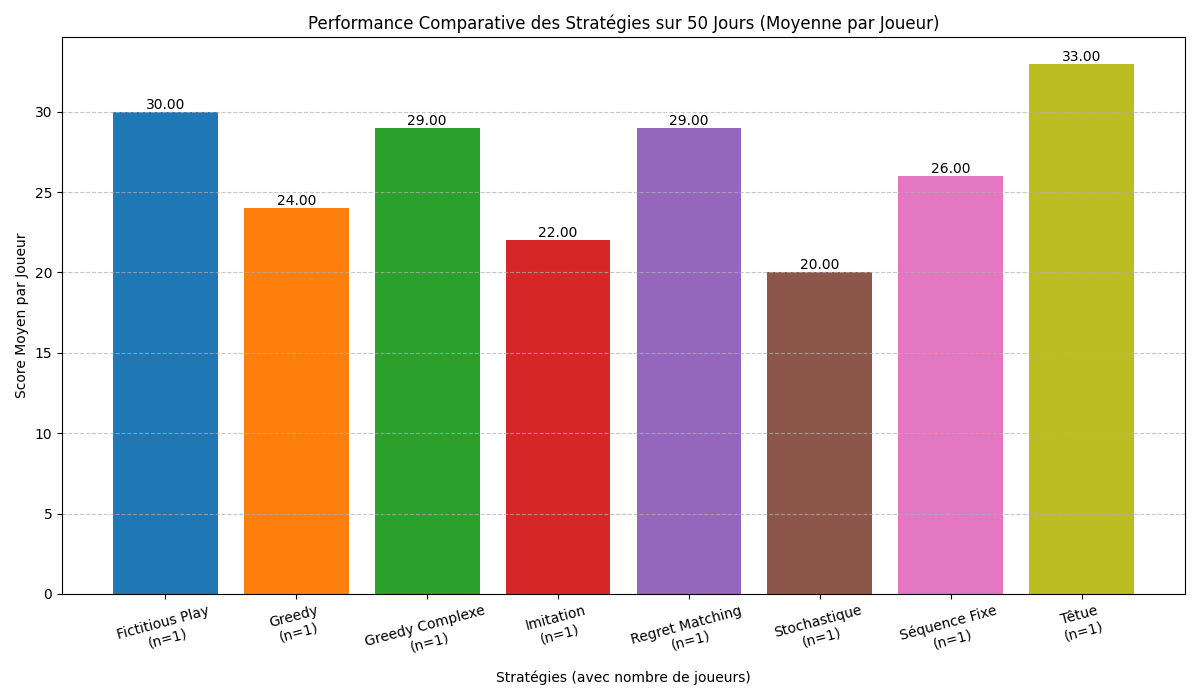
\includegraphics[width=\textwidth]{Figure_1.png}
  \label{fig:figure_1}
  
\end{figure}

\begin{figure}[h]

  \centering
  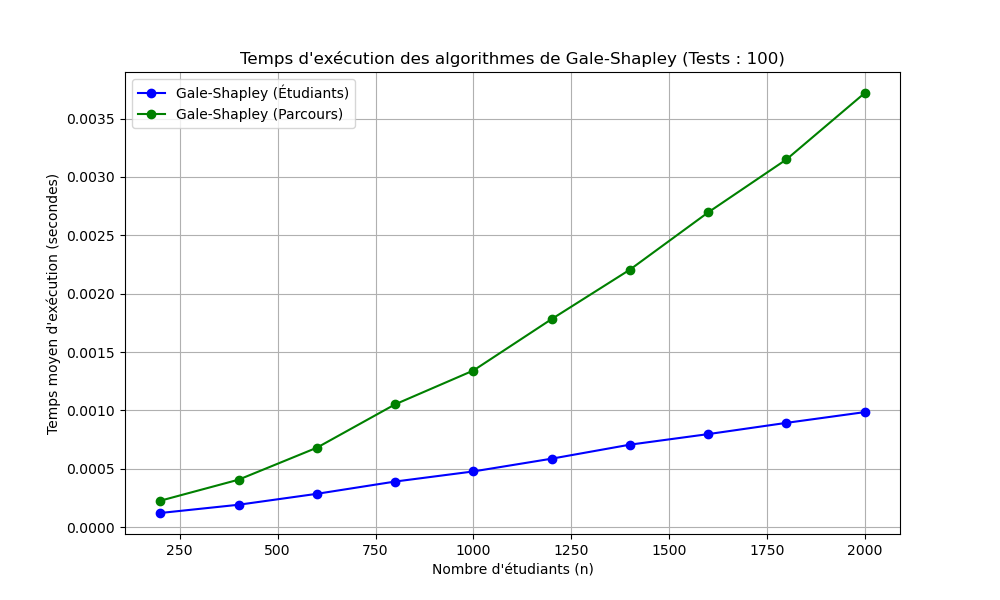
\includegraphics[width=\textwidth]{Figure_100.png}
  \label{fig:figure_100}
  
\end{figure}

\subsection*{Question 10}

Jusqu'à 100 tests effectués, nous obtenons des courbes ressemblant de près à des courbes linéaires, et cela en fonction du nombre d'étudiants impliqués. Les courbes obtenues sont conformes à nos attentes. Comme on peut le remarquer, lorsqu'on effectue un seul test, on voit que les temps d'exécution sont proches des temps moyens obtenus avec une centaine d'itérations, bien que cette fois-ci, on ne peut distinguer l'apparence linéaire des courbes (ce qui n'est pas surprenant, car faire une moyenne permet d'approcher un comportement auquel se rapproche chaque exécution, en terme de temps utilisé) et il suffit de relancer plusieurs fois l'exécution n°2 du menu de notre code pour s'en convaincre, car l'allure de la courbe ne sera jamais exactement la même. Au contraire, lorsque l'on relance avec 100 tests, puisque c'est une moyenne, l'allure de la courbe est toujours similaire et cela nous aide à comprendre les complexités de nos algorithmes.

Nous pouvons noter que les temps d'exécutions pour Gale-Shapley côté étudiant vont de 0.2 ms approximativement pour 200 étudiants à 1.4 ms en moyenne pour 2000 étudiants. Pour l'algorithme côté parcours, nous obtenons environ 0.3 ms comme temps d'exécution avec 200 étudiants et jusqu'à 3.6 ms en moyenne avec 2000 étudiants. Donc, nous voyons clairement que l'algorithme de Gale-Shapley côté étudiant est plus efficace que celui côté parcours, au fur et à mesure que l'on augmente le nombre d'étudiants. De plus, le nombre m de parcours est seulement de 9, donc les deux algorithmes restent très performants, mais avec davantage de parcours considérés, nous obtiendrions des différences bien plus significatives entre les temps d'exécution des deux versions de l'algorithme, car il est susceptible d'y avoir beaucoup plus de réaffectations des étudiants côté parcours et ce qui en découle est que cela augmenterait énormément les temps d'exécution des deux algorithmes et en particulier pour l'algorithme côté parcours.

\section*{Partie 3 : Equité et PL(NE)}

\subsection*{Question 11}

Dans cette étude, nous avons utilisé les fichiers \texttt{PrefEtu.txt} et \texttt{PrefSpe.txt} pour \( n = 11 \) et \( k = 3 \). Notre objectif est de générer un fichier \texttt{.lp} correspondant au Programme Linéaire en Nombres Entiers (PLNE) et de le résoudre à l'aide du solveur Gurobi.

\section{Problème et Modélisation en PLNE}

\subsection{Définitions et Notations}
\begin{itemize}
    \item \( S \) : ensemble des étudiants.
    \item \( P \) : ensemble des parcours.
    \item \( x_{i,j} \) : variable binaire indiquant si l’étudiant \( i \) est affecté au parcours \( j \) :
    \[
    x_{i,j} = \begin{cases} 
    1, & \text{si l’étudiant } i \text{ est affecté au parcours } j \\
    0, & \text{sinon}
    \end{cases}
    \]
    \item \( U_{i,j} \) : score de Borda attribué par l’étudiant \( i \) au parcours \( j \).
    \item \( m \) : nombre total de parcours et \( k \) le nombre maximal de choix considérés.
\end{itemize}

\subsection{Formulation PLNE}
\textbf{Contraintes :}
\begin{enumerate}
    \item \textbf{Chaque étudiant est affecté à un seul parcours} :
    \[
    \sum_{j \in P} x_{i,j} = 1, \quad \forall i \in S
    \]
    \item \textbf{Respect des capacités des parcours} :
    \[
    \sum_{i \in S} x_{i,j} \leq C_j, \quad \forall j \in P
    \]
    \item \textbf{Affectation dans les \( k \) premiers choix} :
    \[
    \sum_{j \in P : U_{i,j} \geq m - k} x_{i,j} = 1, \quad \forall i \in S
    \]
    \item \textbf{Variables binaires} :
    \[
    x_{i,j} \in \{0,1\}, \quad \forall i \in S, \forall j \in P
    \]
\end{enumerate}

\subsection{Génération du fichier LP avec Python}
Le modèle PLNE est généré à l’aide de la fonction \texttt{generate\_lp\_file\_k}, qui prend en entrée les préférences des étudiants et des parcours, ainsi que les capacités des parcours et le nombre maximal de choix \( k \) pour chaque étudiant.


Ce fichier LP est ensuite résolu à l'aide de Gurobi pour trouver une solution qui respecte les contraintes d'affectation, de capacité et de choix parmi les \( k \) premiers choix des étudiants.

\subsection{Résolution avec Gurobi}
Une fois le fichier LP généré, il peut être résolu avec Gurobi pour déterminer l’affectation optimale des étudiants aux parcours, en respectant les contraintes mentionnées.

\subsection{Analyse des Résultats}
Une fois la solution obtenue, nous analyserons l'affectation des étudiants et la capacité de chaque parcours. Nous examinerons également l'utilité moyenne et minimale des étudiants pour évaluer la qualité de la solution.


\section{Génération du fichier \texttt{.lp}}
Nous avons écrit une fonction permettant de générer un fichier \texttt{.lp} représentant notre problème d'affectation. La méthode suit les étapes suivantes :
\begin{enumerate}
    \item Définition des variables \( x_{i,j} \), représentant l'affectation de l'étudiant \( i \) au parcours \( j \).
    \item Ajout des contraintes :
    \begin{itemize}
        \item Chaque étudiant est affecté à un seul parcours.
        \item Respect des capacités des parcours.
        \item Le choix des étudiants respecte les \( k \) premiers choix.
    \end{itemize}
    \item Maximisation de la fonction objective : maximiser les scores de Borda.
\end{enumerate}


\subsection*{Question 12}

Nous avons utilisé la fonction \texttt{generate\_lp\_file\_k}. Après l'exécution de cette fonction, nous avons trouvé les contraintes dans le fichier \texttt{affectation\_k.lp}.

Ensuite, nous avons exécuté la commande suivante : 

\[
\texttt{gurobi\_cl ResultFile=solution.sol affectation\_k.lp}
\]

Les résultats obtenus sont les suivants :

\begin{quote}
Model is infeasible\\
Best objective -, best bound -, gap -\\
Unable to retrieve attribute 'X'
\end{quote}

Cela signifie qu'il n'y a pas de solution pour \( k = 3 \).

\subsection*{Question 13}

À l'aide de la fonction \texttt{find\_min\_k}, nous avons trouvé la valeur minimale de \( k \) permettant à tous les étudiants d'obtenir un de leurs \( k \) premiers choix dans les affectations pour les Masters. Echec à k=4, et affectation stable à partir de k=5, donc il est possible d'obtenir au moins une affectation stable à partir de ce kmin.


\subsection*{Maximisation de l'utilité minimale des étudiants}

Nous cherchons à maximiser l'utilité minimale des étudiants pour un \( k \) donné. Le problème est formulé sous forme d'un Programme Linéaire en Nombres Entiers (PLNE) avec les contraintes suivantes :

\begin{enumerate}
    \item \textbf{Affectation unique de chaque étudiant} :
    Chaque étudiant \( i \) doit être affecté à un seul parcours parmi ses \( k \) premiers choix. Cela se traduit par la contrainte suivante :
    \[
    \sum_{j \in P_i^k} x_{i,j} = 1, \quad \forall i \in S
    \]
    où \( P_i^k \) est l'ensemble des \( k \) premiers choix de l'étudiant \( i \), et \( x_{i,j} \) est une variable binaire indiquant si l'étudiant \( i \) est affecté au parcours \( j \).

    \item \textbf{Respect des capacités des parcours} :
    La capacité de chaque parcours \( j \) doit être respectée, c'est-à-dire que le nombre d'étudiants affectés à ce parcours ne doit pas dépasser sa capacité. La contrainte est formulée comme suit :
    \[
    \sum_{i \in S} x_{i,j} \leq C_j, \quad \forall j \in P
    \]
    où \( C_j \) est la capacité du parcours \( j \).

    \item \textbf{Maximisation de l'utilité minimale} :
    L'objectif est de maximiser l'utilité minimale des étudiants. La contrainte relative à l'utilité minimale est la suivante :
    \[
    \sum_{j \in P_i^k} U_{i,j} \cdot x_{i,j} \geq U_{\min}, \quad \forall i \in S
    \]
    où \( U_{i,j} \) est le score de Borda combiné pour l'étudiant \( i \) et le parcours \( j \), et \( U_{\min} \) est la variable représentant l'utilité minimale que nous cherchons à maximiser.

    \item \textbf{Objectif} :
    L'objectif du problème est de maximiser l'utilité minimale \( U_{\min} \).
    \[
    \text{Maximiser } U_{\min}
    \]
\end{enumerate}

Nous avons utilisé \texttt{PULP} en utilisant la méthode \texttt{PULP\_CBC\_CMD}. Le résultat renvoie l'affectation optimale des étudiants aux parcours ainsi que l'utilité minimale atteinte.

\textbf{Remarque :} Dans la solution obtenue, chaque affectation de l'étudiant à un parcours est représentée par \( x_{i,j} = 1 \), indiquant que l'étudiant \( i \) est affecté au parcours \( j \), et l'utilité minimale obtenue correspond à la valeur de \( U_{\min} \).

Les résultats renvoyés sont les suivants :

\begin{quote}
Votre choix : 5\\
Aucune solution trouvée pour \( k = 1 \), tentative avec \( k = 2 \)\\
Aucune solution trouvée pour \( k = 2 \), tentative avec \( k = 3 \)\\
Aucune solution trouvée pour \( k = 3 \), tentative avec \( k = 4 \)\\
Aucune solution trouvée pour \( k = 4 \), tentative avec \( k = 5 \)\\
Solution trouvée pour \( k = 5 \)\\
Le plus petit \( k \) pour lequel la solution est faisable est : 5
\end{quote}

Afin de maximiser l'utilité minimale des étudiants, nous avons utilisé la fonction \texttt{maximize\_min\_utility}, qui, à l'aide de la fonction \texttt{score\_borda\_combined} (fonction renvoyant une matrice contenant l'ensemble des sommes des scores étudiants et parcours), nous a permis de déterminer l'utilité minimale la plus haute, atteinte.

L'affichage obtenu est le suivant :

\begin{quote}
Plus petit \( k \) trouvé : 5\\
Affectation optimale : \{(0, 8): 1.0, (1, 4): 1.0, (2, 0): 1.0, (3, 0): 1.0, (4, 1): 1.0, (5, 7): 1.0, (6, 5): 1.0, (7, 2): 1.0, (8, 6): 1.0, (9, 8): 1.0, (10, 3): 1.0\}\\
Utilité minimale atteinte : 8.0
\end{quote}

Les valeurs \texttt{1.0} indiquent que les affectations des étudiants aux parcours ont bien été réalisées. Sinon, elles seraient à \texttt{0.0} (mais l'algorithme renvoie directement la solution trouvée, donc il n'y a pas de \texttt{0.0}). Les couples sont sous la forme (étudiant, parcours), et l'utilité minimale trouvée est de 8 pour \( k = 5 \) (\( k_{\text{min}} \)). Cela signifie que l'étudiant le moins satisfait a une utilité minimale de 8, et tous les autres étudiants ont au moins 8 comme utilité minimale également.




\section*{Modèle de Programmation Linéaire pour Maximiser l'Efficacité Totale avec Équité}


\subsection*{Question 14}
\subsection{PLNE pour maximiser la somme des utilités}

Nous devons écrire un \textbf{Programme Linéaire en Nombres Entiers (PLNE)} permettant de maximiser la somme des utilités des étudiants et des parcours.

\subsubsection{Modèle PLNE}

\textbf{Variables de décision :}  
\[
x_{i,j} \in \{0,1\}
\]
où \( x_{i,j} = 1 \) si l'étudiant \( i \) est affecté au cours \( j \), sinon \( 0 \).

\textbf{Objectif :}  
Maximiser la somme des utilités (score Borda combiné) :

\[
\max \sum_{i=1}^{n} \sum_{j \in P_i} s_{i,j} \cdot x_{i,j}
\]

où \( s_{i,j} \) est le score Borda combiné du couple \( (i,j) \) et \( P_i \) est l’ensemble des \( k \) premiers choix de l’étudiant \( i \).

\textbf{Contraintes :}
\begin{itemize}
    \item \textbf{Chaque étudiant est affecté à un seul cours}  
    \[
    \sum_{j \in P_i} x_{i,j} = 1, \quad \forall i \in \{1, ..., n\}
    \]
    \item \textbf{Capacité des parcours respectée}  
    \[
    \sum_{i: j \in P_i} x_{i,j} \leq c_j, \quad \forall j \in \{1, ..., m\}
    \]
    \item \textbf{Les variables sont binaires}  
    \[
    x_{i,j} \in \{0,1\}, \quad \forall i, j
    \]
\end{itemize}

\subsubsection{Résolution avec Gurobi}

Nous avons résolu le PLNE pour différentes valeurs de \( k \) :

\begin{table}[h]
    \centering
    \begin{tabular}{|c|c|c|c|c|}
        \hline
        \( k \) & Utilité totale atteinte & Utilité moyenne atteinte & Utilité minimale & Valeur objective \\
        \hline
        5 & 131 & 6.55 & 2 & 129 \\
        6 & 144 & 7.2 & 7 & 144 \\
        7 & 153 & 7.65 & 10 & 153 \\
        8 & 153 & 7.65 & 10 & 153 \\
        9 & 153 & 7.65 & 10 & 153 \\
        \hline
    \end{tabular}
    \caption{Résultats de l'optimisation en fonction de \( k \)}
\end{table}

\textbf{Interprétation :}
\begin{itemize}
    \item L’utilité totale \textbf{augmente avec \( k \)}, mais \textbf{se stabilise à \( k = 7 \)}.
    \item À partir de \( k = 7 \), \textbf{l’utilité minimale atteint 10}, garantissant une meilleure équité.
    \item \textbf{\( k = 7 \) est donc un bon choix}, car il maximise l’utilité et assure une équité entre étudiants.
\end{itemize}

\textbf{Réponse finale :}
\begin{itemize}
    \item \textbf{Utilité moyenne obtenue :} \( 7.65 \)
    \item \textbf{Utilité minimale obtenue :} \( 10 \)
    \item \textbf{Valeur optimale de \( k \) choisie :} \( 7 \)
\end{itemize}

Resultat obtenu:
\begin{tabular}{|c|l|}
\hline
Parcours & Etudiant(s) \\
\hline
0 & [4, 5] \\
\hline
1 & [10] \\
\hline
2 & [7] \\
\hline
3 & [3] \\
\hline
4 & [9] \\
\hline
5 & [0] \\
\hline
6 & [8] \\
\hline
7 & [6] \\
\hline
8 & [1, 2] \\
\hline
\end{tabular}

\subsection*{Question 15}

Nous souhaitons maximiser la somme des utilités combinées des étudiants et des parcours tout en garantissant une utilité minimale pour chaque étudiant. Le modèle de programmation linéaire est défini comme suit :

\subsection*{Variables de décision}

\begin{itemize}
    \item $x_{ij} = 
        \begin{cases} 
            1 & \text{si l'étudiant } i \text{ est affecté au parcours } j \\
            0 & \text{sinon}
        \end{cases}$
    \item $U_{\min} \geq 0$ : Utilité minimale garantie pour chaque étudiant.
\end{itemize}

\subsection*{Paramètres}

\begin{itemize}
    \item $n$ : Nombre d'étudiants.
    \item $m$ : Nombre de parcours.
    \item $k$ : Nombre de premiers choix considérés pour chaque étudiant.
    \item $S_{ij}$ : Score de Borda combiné de l'étudiant $i$ pour le parcours $j$.
    \item $C_j$ : Capacité maximale du parcours $j$.
\end{itemize}

\subsection*{Fonction Objectif}

Nous maximisons la somme des utilités combinées des étudiants et des parcours, en ajoutant un poids pour garantir l'équité :

\[
\max \left( \sum_{i=1}^{n} \sum_{j \in P_i^k} S_{ij} \cdot x_{ij} + U_{\min} \right)
\]

où $P_i^k$ est l'ensemble des $k$ premiers choix de l'étudiant $i$.

\subsection*{Contraintes}

\begin{enumerate}
    \item \textbf{Affectation unique des étudiants :}
    \[
    \sum_{j \in P_i^k} x_{ij} = 1, \quad \forall i \in \{1, \dots, n\}
    \]

    \item \textbf{Respect des capacités des parcours :}
    \[
    \sum_{\substack{i=1 \\ j \in P_i^k}}^{n} x_{ij} \leq C_j, \quad \forall j \in \{1, \dots, m\}
    \]

    \item \textbf{Utilité minimale garantie pour chaque étudiant :}
    \[
    \sum_{j \in P_i^k} S_{ij} \cdot x_{ij} \geq U_{\min}, \quad \forall i \in \{1, \dots, n\}
    \]

    \item \textbf{Variables binaires :}
    \[
    x_{ij} \in \{0, 1\}, \quad \forall i \in \{1, \dots, n\}, \quad \forall j \in P_i^k
    \]
\end{enumerate}

En appliquant la fonction \texttt{maximize\_utility\_and\_fairness} avec les paramètres suivants :

\begin{itemize}
    \item \textbf{Valeur de } $k$ : 5
\end{itemize}

Nous obtenons les résultats suivants :

\begin{itemize}
    \item \textbf{Utilité totale atteinte} : 131.0
    \item \textbf{Utilité moyenne atteinte} : 6.55
    \item \textbf{Utilité minimale des étudiants} : 8.0
\end{itemize}

\section*{Conclusion}

L'application de ce modèle d'optimisation a permis de maximiser l'efficacité totale tout en garantissant une certaine équité entre les étudiants. L'utilité moyenne atteinte est de 6.55, ce qui reflète une distribution globale satisfaisante des affectations. Cependant, l'utilité minimale des étudiants reste relativement basse à 2.0, ce qui indique qu'au moins un étudiant bénéficie d'une affectation loin de ses préférences optimales. Cela souligne la difficulté d'équilibrer parfaitement efficacité et équité dans ce type de problème d'affectation.


\section*{Comparaison des différentes solutions obtenues}

\subsection*{Question 16}

Ensemble des affectations trouvées pour chaque question :

\begin{tabular}{|c|l|}
\hline
Question & Affectations \\
\hline
Q3 & 0: [3, 5], 1: [4], 2: [9], 3: [8], 4: [10], 5: [0], 6: [1], 7: [7], 8: [2, 6] \\
\hline
Q4 & 0: [5, 3], 1: [4], 2: [9], 3: [8], 4: [10], 5: [1], 6: [0], 7: [7], 8: [6, 2] \\
\hline
Q13 & 0: [2, 3], 1: [4], 2: [7], 3: [10], 4: [1], 5: [6], 6: [8], 7: [5], 8: [0, 9] \\
\hline
Q14 & 0: [4, 5], 1: [10], 2: [7], 3: [3], 4: [9], 5: [0], 6: [8], 7: [6], 8: [1, 2] \\
\hline
Q15 & 0: [7, 10], 1: [4], 2: [6], 3: [9], 4: [5], 5: [0], 6: [1], 7: [3], 8: [2, 8] \\
\hline
\end{tabular}


Nous avons plusieurs solutions :
\begin{itemize}
    \item \textbf{Gale-Shapley côté étudiants (Résultats Q3)} : C'est la solution obtenue par l'algorithme Gale-Shapley basé sur les préférences des étudiants.
    \item \textbf{Gale-Shapley côté parcours (Résultats Q4)} : C'est la solution obtenue par l'algorithme Gale-Shapley basé sur les préférences des parcours.
    \item \textbf{Solutions des questions 13, 14 et 15} : Ces solutions proviennent de l'optimisation visant à maximiser l'utilité totale tout en respectant certaines contraintes supplémentaires.
\end{itemize}

Nous allons comparer ces solutions selon les critères suivants :
\begin{itemize}
    \item \textbf{Stabilité} (existe-t-il des paires instables ?)
    \item \textbf{Utilité moyenne} (la moyenne des utilités des étudiants)
    \item \textbf{Utilité minimale} (l'utilité minimale parmi les étudiants)
\end{itemize}

\subsection*{1. Stabilité}

Selon la nature de l'algorithme \textbf{Gale-Shapley}, il garantit que les paires retournées sont stables. Par conséquent, les solutions obtenues dans la \textbf{Q3} et la \textbf{Q4} doivent être stables.

\begin{itemize}
    \item \textbf{Résultats Q3 (GS côté étudiants)} : La solution est stable par définition.
    \item \textbf{Résultats Q4 (GS côté parcours)} : La solution est stable par définition.
    \item \textbf{Résultats Q13} : Instable d'après le résultat obtenu.
    \item \textbf{Résultats Q14} : Instable d'après le résultat obtenu.
    \item \textbf{Résultats Q15} : Instable d'après le résultat obtenu.
\end{itemize}

Si nous souhaitons trouver des affectations stables (contrainte), il faut donc utiliser l'algorithme de Gale-Shapley, mais néanmoins, cet algorithme (côté étudiant comme côté parcours) ne garantit pas l'équité et l'efficacité.


\subsection*{2. Utilité moyenne}

L'utilité moyenne représente la satisfaction globale des étudiants. Une utilité moyenne plus élevée indique une plus grande satisfaction des étudiants.


\subsection*{Méthode}
Pour chaque étudiant, on regarde où se trouve le parcours qui lui a été attribué dans sa liste de préférences.

\subsection*{Gale-Shapley côté étudiants}


\begin{tabular}{|c|c|c|c|}
\hline
Étudiant & Parcours attribué & Liste de préférences(coté Etu) & Classement (8 = meilleur choix) \\
\hline
3 & 0 & [6, 5, 7, 0, 8, 4, 3, 1, 2] & 5 \\
5 & 0 & [0, 7, 4, 2, 8, 3, 1, 6, 5] & 8 \\
4 & 1 & [1, 6, 7, 5, 0, 2, 4, 8, 3] & 8 \\
9 & 2 & [2, 6, 5, 8, 3, 1, 4, 7, 0] & 8 \\
8 & 3 & [5, 7, 6, 2, 8, 3, 0, 1, 4] & 3 \\
10 & 4 & [6, 4, 0, 8, 3, 1, 5, 2, 7] & 7 \\
0 & 5 & [5, 7, 6, 8, 3, 2, 0, 1, 4] & 8 \\
1 & 6 & [6, 5, 0, 4, 7, 2, 8, 3, 1] & 8 \\
7 & 7 & [7, 0, 4, 2, 8, 3, 1, 6, 5] & 8 \\
2 & 8 & [4, 0, 7, 2, 8, 3, 1, 6, 5] & 4 \\
6 & 8 & [5, 7, 6, 2, 8, 3, 0, 1, 4] & 4 \\
\hline
\end{tabular}

\begin{tabular}{|c|c|c|c|}
\hline
Étudiant & Parcours attribué & Liste de préférences(coté Spe) & Classement (10 = meilleur choix) \\
\hline
3 & 0 & [7, 9, 5, 4, 3, 1, 0, 10, 6, 8, 2] & 6 \\
5 & 0 & [7, 9, 5, 4, 3, 1, 0, 10, 6, 8, 2] & 8 \\
4 & 1 & [7, 5, 9, 4, 3, 1, 0, 10, 8, 6, 2] & 7 \\
9 & 2 & [3, 9, 5, 4, 7, 6, 1, 0, 10, 8, 2] & 9 \\
8 & 3 & [7, 9, 5, 4, 3, 1, 0, 6, 10, 8, 2] & 1 \\
10 & 4 & [10, 3, 0, 4, 5, 6, 7, 8, 9, 1, 2] & 10 \\
0 & 5 & [1, 0, 3, 4, 5, 6, 7, 2, 9, 10, 8] & 9 \\
1 & 6 & [0, 1, 3, 4, 5, 6, 7, 2, 8, 10, 9] & 9 \\
7 & 7 & [7, 6, 9, 5, 4, 3, 1, 0, 10, 8, 2] & 10 \\
2 & 8 & [1, 0, 3, 4, 5, 6, 7, 2, 9, 10, 8] & 3 \\
6 & 8 & [1, 0, 3, 4, 5, 6, 7, 2, 9, 10, 8] & 5 \\
\hline
\end{tabular}

\subsubsection*{Satisfaction moyenne des étudiants (côté étudiants) en fusionnant les classement de deux tableau au-dessus}
\[
\frac{11 + 16 + 15 + 17 + 4 + 17 
+ 17 + 17 + 18 + 7 + 9}{20} = 7.4
\]

\subsection*{Gale-Shapley côté parcours}

\begin{tabular}{|c|c|c|c|}
\hline
Étudiant & Parcours attribué & Liste de préférences(coté Spe) & Classement (10 = meilleur choix) \\
\hline
5 & 0 & [7, 9, 5, 4, 3, 1, 0, 10, 6, 8, 2] & 8 \\
3 & 0 & [7, 9, 5, 4, 3, 1, 0, 10, 6, 8, 2] & 6 \\
4 & 1 & [7, 5, 9, 4, 3, 1, 0, 10, 8, 6, 2] & 7 \\
9 & 2 & [3, 9, 5, 4, 7, 6, 1, 0, 10, 8, 2] & 9 \\
8 & 3 & [7, 9, 5, 4, 3, 1, 0, 6, 10, 8, 2] & 1 \\
10 & 4 & [10, 3, 0, 4, 5, 6, 7, 8, 9, 1, 2] & 10 \\
1 & 5 & [1, 0, 3, 4, 5, 6, 7, 2, 9, 10, 8] & 10 \\
0 & 6 & [0, 1, 3, 4, 5, 6, 7, 2, 8, 10, 9] & 10 \\
7 & 7 & [7, 6, 9, 5, 4, 3, 1, 0, 10, 8, 2] & 10 \\
6 & 8 & [1, 0, 3, 4, 5, 6, 7, 2, 9, 10, 8] & 5 \\
2 & 8 & [1, 0, 3, 4, 5, 6, 7, 2, 9, 10, 8] & 3 \\
\hline
\end{tabular}

\begin{tabular}{|c|c|c|c|}
\hline
Étudiant & Parcours attribué & Liste de préférences(coté Etu) & Classement (8 = meilleur choix) \\
\hline
5 & 0 & [0, 7, 4, 2, 8, 3, 1, 6, 5] & 8 \\
3 & 0 & [6, 5, 7, 0, 8, 4, 3, 1, 2] & 5 \\
4 & 1 & [1, 6, 7, 5, 0, 2, 4, 8, 3] & 8 \\
9 & 2 & [2, 6, 5, 8, 3, 1, 4, 7, 0] & 8 \\
8 & 3 & [5, 7, 6, 2, 8, 3, 0, 1, 4] & 3 \\
10 & 4 & [6, 4, 0, 8, 3, 1, 5, 2, 7] & 7 \\
1 & 5 & [6, 5, 0, 4, 7, 2, 8, 3, 1] & 7 \\
0 & 6 & [5, 7, 6, 8, 3, 2, 0, 1, 4] & 6 \\
7 & 7 & [7, 0, 4, 2, 8, 3, 1, 6, 5] & 8 \\
6 & 8 & [5, 7, 6, 2, 8, 3, 0, 1, 4] & 4 \\
2 & 8 & [4, 0, 7, 2, 8, 3, 1, 6, 5] & 4 \\
\hline
\end{tabular}

\subsubsection*{Satisfaction moyenne des étudiants (côté parcours) en fusionnant les classement de deux tableau au-dessus}
\[
\frac{16 + 11 + 15 + 17 + 4 + 17 + 17 + 16 + 18 + 9 + 7}{20} = 7.35
\]

\begin{itemize}
    \item \textbf{Résultats Q3} : Utilité moyenne 7.4
    \item \textbf{Résultats Q4} : Utilité moyenne 7.35
    \item \textbf{Résultats Q13} : Utilité moyenne 6.55
    \item \textbf{Résultats Q14} : Utilité moyenne 7.65
    \item \textbf{Résultats Q15} : Utilité moyenne 6.45
\end{itemize}

La solution \textbf{Q14} a la plus haute utilité moyenne, indiquant que les étudiants sont plus satisfaits, comparé aux autres solutions. Donc la meilleure solution est k=7 pour maximiser l'utilité moyenne.

\subsection*{3. Utilité minimale}

L'utilité minimale est la valeur de l'utilité la plus faible parmi tous les étudiants. Idéalement, on souhaite que cette valeur soit aussi élevée que possible afin de garantir l'équité.

\begin{itemize}
    \item \textbf{Résultats Q3} : Utilité minimale 4.0
    \item \textbf{Résultats Q4} : Utilité minimale 4.0
    \item \textbf{Résultats Q13} : Utilité minimale 2.0
    \item \textbf{Résultats Q14} : Utilité minimale 10.0
    \item \textbf{Résultats Q15} : Utilité minimale 8.0
\end{itemize}

La solution, \textbf{Q14} a une utilité minimale de 10, ce qui est bien plus équitable que les solutions des autres questions, qui ont des utilités minimales inférieures ou égales à 8.


\subsection*{Conclusion}

\begin{itemize}
    \item \textbf{Stabilité} : Les solutions aux \textbf{Q3} et \textbf{Q4} sont stables (garanties par Gale-Shapley), tandis que les solutions \textbf{Q13}, \textbf{Q14}, et \textbf{Q15} sont plus optimisées, mais peuvent contenir des paires instables.
    \item \textbf{Utilité moyenne} : La solution \textbf{Q14} a la plus grande utilité moyenne, ce qui signifie que les étudiants sont globalement plus satisfaits.
    \item \textbf{Utilité minimale} : La solution \textbf{Q14} a la plus grande utilité minimale, ce qui est plus équitable que les résultats trouvés aux autres questions, qui ont des utilités minimales inférieures ou égales à 8, signifiant que l'évaluation de l'affectation pour l'étudiant ayant le plus petit score pour celle-ci, selon la position dans ses préférences au parcours auquel il est associé et de la position de l'étudiant dans les préférences de ce parcours, est meilleure que l'évalutation du plus petit score obtenu pour chacune des autres questions. Autrement dit, la pire affectation de toutes obtient un score plus élevé avec les affectations trouvées à la \textbf{Q14} qu'avec les autres questions.
\end{itemize}

En résumé, la solution obtenue à la \textbf{Q14} est la plus intéressante, bien qu'il puisse y avoir quelques paires instables, elle améliore l'utilité des étudiants et est plus équitable que les affectations données par les algorithmes de Gale-Shapley. Donc, hormis la contrainte de stabilité, la solution trouvée à cette question est meilleure en tout point.

\end{document}
